\chapter{evaluation}\label{chapter:evaluation}

To evaluate the project researchers at both Imperial College London and Kings College London have been consulted for feedback. Since the evaluation group is relatively small (~10 users) the focus of the interviews was to gain insights by having a conversation with them. The best feedback received came from just speaking with the researchers and trying to get a glimpse into their way of seeing things. Having said that the interviews were also guided with some more rigidly defined questions which give some quantitative insight into the project. Each part of the plugin has been evaluated separately.

\section{Scan Simulation}
For the scan simulation part of the project feedback from the users was needed firstly on whether this was a useful feature for them. Then limitations of the current implementation needed to be found: are all the scan customization parameters that they expect avaialable? Are there any more scanning artefacts that need to be simulated?

The potential users were asked 'How useful is this feature for you?' and their responses are shown below in figure \ref{fig:graph_scansimulation_1}.

\begin{figure}[h]
    \centering
	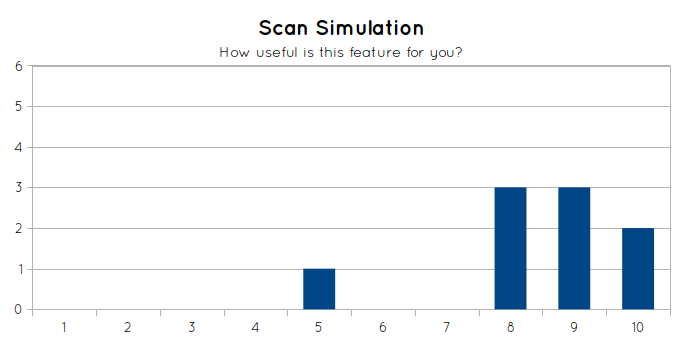
\includegraphics[width=0.6\textwidth]{images/evaluation/graph_scan_simulation_1.png}
    \caption{1 is useless. 10 is very useful.}\label{fig:graph_scansimulation_1}
\end{figure}

The majority of users thought that this feature would be of use for them. The one notable exception on the graph was due to concerns that the complexity of the simulation currently implemented is a far cry from that required. More on that shortly.

The users were then asked 'Does it include all of the parameters that you would expect?' and 'Is the simulation realistic enough?' to get an idea of what other features need to be implemented. Their responses are shown in figure \ref{fig:graph_scan_simulation23}.

\begin{figure}[H]
  \centering
  \begin{subfigure}[b]{0.5\textwidth}
    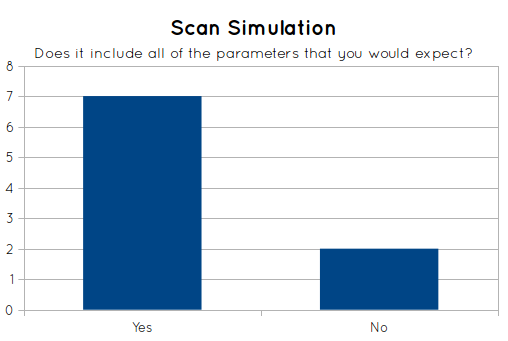
\includegraphics[width=\textwidth]{images/evaluation/graph_scan_simulation_2.png}
    %\caption{Variation 1}
    %\label{fig:graph_scansimulation_2}
  \end{subfigure}%
  ~ %add desired spacing between images, e. g. ~, \quad, \qquad, \hfill etc.
    %(or a blank line to force the subfigure onto a new line)
  \begin{subfigure}[b]{0.5\textwidth}
    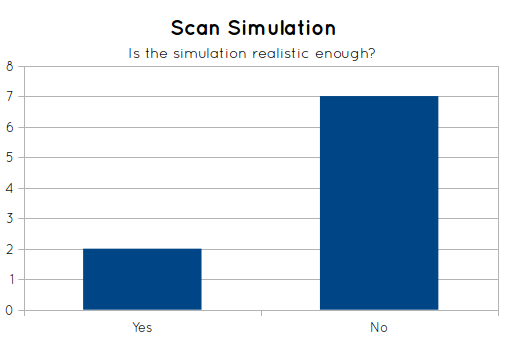
\includegraphics[width=\textwidth]{images/evaluation/graph_scan_simulation_3.png}
    %\caption{Variation 2}
    %\label{fig:graph_scansimulation_3}
  \end{subfigure}
  \caption{}\label{fig:graph_scan_simulation23}
\end{figure}

For the most part the researchers felt that the control they have over the scan configuration was enough. One suggested that instead of specifying the value in pixels, which was a natural unit to use when dealing with a reconstructed volume, it would be good to have the option to specify mm instead, which more closely matches a MRI scanner. Another point which was raised was that the ability to specify a scan plane by selecting two points in the volume was something that they would like as it gives them finer directional control and the ability to more easily setup shorter scans.

The question about whether the simulation was realistic enough provoked the largest response. As it turns out there are many things that researchers would like to see integrated. Here they are <insert here>.... look at sheets.

This raises the question of how much realism needs to be simulated to effectively test reconstruction algorithms. Highly realistic MRI simulation has been done before and tools, such as MRiLab\cite{mrilab}, allow the user to experiment with different scan sequences, coils and more. Whether this level of detail is needed to accurately test a reconstruction algorithm requires more research.

\section{Reconstruction}
Opinion. Landmarks. Time to do it. Feedback. Different feedback from different points of view.

\section{Visualization}
Three things. Understand. Clear. Configurable.

% General Format -> What we wanted to find out. Go through each question. For those that are quantitative give us a graph. For those that aren't then talk about What they said.